%% chapter 1

\chapter{绪论}
\section{研究背景}
  在病毒或细菌感染期间,免疫因子会在人体中释放,通常会导致组织发炎并导致严重的疾病行为,例如食欲不振,嗜睡,退出正常的社交活动,疲劳,探索力下降等。人们认为疾病行为是由可溶性促炎性细胞因子(IL-1、$TNF-\alpha$、IL-6等)触发的,该因子由感染部位的免疫细胞产生,并会对神经内分泌系统,特别是下丘脑-垂体-肾上腺(HPA)轴\cite{chrousos1995hypothalamic,shanks2000early}产生深远的影响。

  HPA轴是体内的压力反应中心,连接中枢神经系统(CNS)和内分泌系统,其在炎症状态下的调节过程如\ref{fig:HPA}所示。作为HPA轴组成部分的垂体,在炎症事件调节过程中起到重要的作用。由炎症事件诱导的细胞因子(IL1,IL6,TNF-$\alpha$,IFN-$\gamma$)通常循环至垂体前叶,并主要作用于垂体的促肾上腺皮质激素,从而促进释放抗炎激素,例如肾上腺皮质激素(ACTH)。ACTH被携带到肾上腺并作用于ACTH受体,从而上调肾上腺皮质肾上腺皮质细胞中皮质醇的释放。随后,皮质醇在下丘脑和垂体在HPA轴上产生负反馈,以抑制促炎性细胞因子的进一步合成和释放。此外,卵泡细胞代表垂体前叶中唯一的非内分泌细胞类型,并释放可能潜在影响垂体局部激素产生的IL1和IL6,从而构成调节炎症反应的复杂系统。

\begin{figure}[!htb]
  \centering
  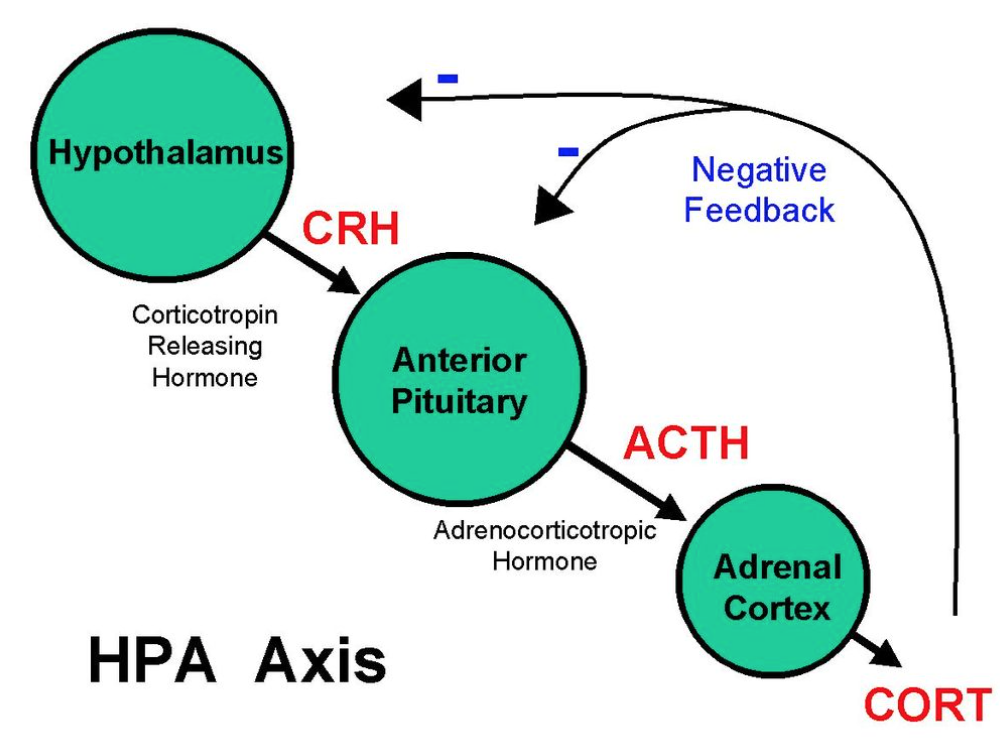
\includegraphics[width=0.6\textwidth]{figs/HPA.png}
  \caption{炎症状态下的HPA轴}
  \label{fig:HPA}
\end{figure}

\section{研究现状与研究内容}
  以往探究垂体在中枢神经内分泌炎症调节过程中作用的研究\cite{chrousos1995hypothalamic,shanks2000early}都没有涉及到单细胞转录层级,没有揭示垂体内部各类细胞在中枢神经内分泌炎症调解过程中的角色以及内在调控因子。

  近几年随着单细胞RNA测序技术的发展\cite{svensson2018exponential},研究人员开始从单细胞转录组水平探究垂体相关的一些问题\cite{chen2020single,cheung2018single,ho2020single,fletcher2019cell},但这些工作主要关注于某个发育过程中的静态分类问题,很少有研究使用单细胞转录组测序来进行动态功能研究。

  在这项研究中,我们主要关注不同的垂体细胞如何响应炎症刺激。我们将基于病毒或细菌感染建立炎症小鼠模型,并主要使用单细胞转录组测序以及数据分析和数据挖掘来找出炎症、垂体和激素之间的关系,动态炎症研究将成为我们实验中最重要的部分。这项研究可以使我们对人体对病毒或细菌感染的免疫防御具有更清晰的认识。更重要的是,它具有非常重要的临床意义,我们希望获得用于免疫诊断的特定标记。此外,这项研究也可以为我们提供关于单细胞转录组测序技术应用的新思路。

\section{研究结果}
  在这项研究中,我们的主要贡献有:(1)建立了一个涉及多种免疫刺激剂、多尺度给药剂量与恢复时程的小鼠炎症模型,并在单细胞水平上提供了其垂体细胞测序数据。(2)揭示了不同种类垂体细胞在参与中枢神经内分泌炎症调节的过程中的转录水平差异,表明其在炎症调节过程中扮演不同的角色。(3)发现了一类在不同种类垂体细胞中统一表达的转录因子,表明其在垂体参与中枢神经内分泌炎症调节过程中的重要地位。

  文章结构安排如下:第二章介绍单细胞测序以及基因调控网络(GRN)的相关工作;第三章介绍单细胞RNA测序数据处理流程;第四章介绍SCENIC算法原理;第五章介绍使用GRN对小鼠垂体单细胞测序数据进行分析;第六章总结了我们的结论并对未来的工作进行了展望。

